\documentclass{article}
\def\npart {2}
\def\nterm {LMS Summer School}
\def\nyear {2021}
\def\nlecturer {Sophie Morier-Genoud : Sorbonne Universite, Paris}
\def\ncourse {Arithmetic and combinatorics of Conway-Coxeter frieze patterns}

\input{header}

\begin{document}
  \maketitle

\section{Overview and }
\subsection{Continued fraction}
Let's take $x \in \R$ and we can say, $a < x < a + 1$ where $a \in \Z$. Now we write, $x = a + \frac{1}{x'}$, $x' > 1$.

\begin{align*}
  x = a + \frac{1}{x'} \\
  &= a + \frac{1}{a' + \frac{1}{x''}}\\
  &\vdots\\
  &= a_1 + \frac{1}{a_2 + \frac{1}{a_3 + \frac{1}{\ddots}}}
\end{align*}
where $a_1 \in \Z$ and $a_i \ge 1$ for $\forall i \ge 2$. \\

\begin{nlemma}
  The sequence of $a_i$'s are finite if and only if $x \in \Q$.
\end{nlemma}
\begin{proof}
  If it's finite, it's obvious that it's rational.\\
  Conversely, this is due to Euclid's algorithm. Take $\frac{p}{q} \in \Q$ and then write,
  \begin{align*}
    p &= a_1q + r_1 && 0 \le r_1 \le q\\
    q &= a_2r_1 + r_2 && 0 \le r_2 \le r_1\\
  \end{align*}
\end{proof}
or we can form them by subtracting instead of adding, these make negative expansion (or Hirzebruch-Sung),
$$ x = a_1 - \frac{1}{a_2 - \frac{1}{a_3 - \frac{1}{\ddots}}} $$

\begin{notation}
 $x = [a_1, a_2, \dots]$ means $x$ is a regular continued fraction and $x = \lb a_1, a_2, \dots\rb $ means a negative expansion.
\end{notation}

  Let's take $x \notin \Q$ and consider the golden ratio,\\
  $$ \varphi = [1, 1, 1, 1, 1, 1, 1, \dots] $$
  and now $e$, there is some regularity,
  $$ e = [2, 1, 2, 1, 1, 4, 1, 1, 6, 1, 1, 8, 1, \dots] $$
  and now $\pi$, there is no regularity,
  $$ \pi = [3, 7, 15, 1, 292, 1, 1, \dots] $$

Now consider the generalised continued fraction,
$$ \pi = \frac{4}{1 + \frac{1^2}{2 + \frac{3^2}{2 + \frac{5^2}{\ddots}}}} $$
Now consider the negative expansion,
$$ \lb 2, 2, 2, 2, 2, 2, \dots\rb  $$
This is just one. It may be represented with an infinite sequence.\\

Here are some more examples,
\begin{align*}
  \frac{5}{2} &= [2, 2] = \lb  3, 2 \rb \\
  \frac{10}{3} &= [3, 3] = \lb  4, 2, 2 \rb \\
  \frac{14}{5} &= [2, 1, 3, 1] = \lb  3, 5 \rb \\
  \frac{43}{16} &= [2, 1, 2, 5] = \lb  3, 4, 2, 2, 2, 2 \rb
\end{align*}

\begin{remark}
  To make it unique one can always choose an even number for the length of the sequence. For a regular expansion, we can always assume that it's of even length.
\end{remark}

There is a very natural question, given $x = [a_1, \dots, a_{2m}] = \lb c_1, c_2, \dots c_k \rb $, what is the relationship between $a_i$'s and $c_i$'s?

\subsection{Friezes}
Friezes are from Coxeter in the 1970's. We have the first and last row as 1's. When you have a diamond of numbers,

\begin{figure}[!ht]
\centering
\begin{tabular}{cccccccccccccccccccc}
 1&&1&&1&&1&&1&&1&&1&&1&&1&&1 \\
 &4&&1&&2&&2&&3&&1&&2&&4&&1&\\
 \dots&&3&&1&&3&&5&&2&&1&&7&&3&&\dots\\
 &5&&2&&1&&7&&3&&1&&3&&5&&2&\\
 \dots&&3&&1&&2&&4&&1&&2&&2&&3&&\dots\\
  &1&&1&&1&&1&&1&&1&&1&&1&&1& \\
\end{tabular}
\caption{A frieze pattern}
\end{figure}

and we also have the frieze patter rule, dubbed the unimodular rule, taking a part of the frieze we can create it by saying,
\begin{figure}[!ht]
  \centering
  \begin{tabular}{ccc}
    &b&\\
    a&&d\\
    &c&\\
  \end{tabular}
\end{figure}

and we restrict the entries such that $ad - bc = 1$.
%     b
%  a    d
%     c
% ad - bc = 1

\begin{nthm}[Coxeter]
  Friezes are periodic!
\end{nthm}

We shall consider the width of the frieze, don't count the ones. The example has width of 4 and we can look at the width + 4, we get some perdiodic notion. This means we just need the first `row' to fill the frieze.\\

Furthermore, we now have some sort of glide symmetry. We can form triangles and they repeat themselves. Let's finish the statement

\begin{nthm}[Coxeter]
  Friezes are periodic!
  \begin{itemize}
    \item Width $w \to (w+3)$ is a period.
    \item Invariant under a glide symmetry.
  \end{itemize}
\end{nthm}

\begin{ex}
  Exerises 1,2,3 and 4.
\end{ex}

\textbf{Question 2:} How to get frieze containing only positive integers?\\

\subsection{Triangulation of n-gons}

\begin{ndefi}[Diagonal]
  A line that joins two non-consecutive vertices.
\end{ndefi}

\begin{ndefi}[Triangulation]
  The maximum number of non-intersecting diagonals.
\end{ndefi}
The triangulation is not unique. The number of triangulations is related to the Catalan numbers. For every triangulation, you may two or more triangles on the exterior. We will consider exactly two exterior triangles for the minute,\\
Fix a triangulation with two exterior triangles, if you join two external vertices of these external triangles, then you will intersect every other triangle.\\

If you consider the triangles layed next to eachother like this,
\begin{figure}[!ht]
  \centering
  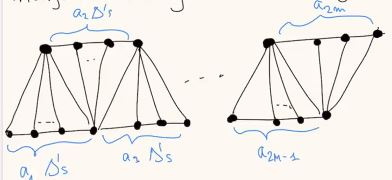
\includegraphics{./figures/L1.2}
  \caption{}
\end{figure}
We can count how many triangles are incidence to the vertex. We shall call this $c_i$ where $i$ is the number of the vertex. If we do this for the 7-gon,
\begin{figure}[!ht]
  \centering
  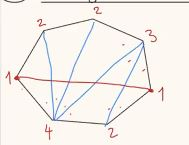
\includegraphics{./figures/L1.3}
  \caption{}
\end{figure}
The sequence $(a_1, a_2, \dots, a_{2n})$ determines the triangulation and the so does the sequence, $(c_1, c_2, \dots)$.

\begin{nthm}
  With this data, we can say that,
  \begin{itemize}
    \item $[a_1, a_2, \dots, a_{2m}] = \lb  c_1, c_2, \dots, c_k \rb $
    \item $(c_1, c_2, \dots, c_n)$ determines a frieze of width $n-3$ containing only positive integers.
  \end{itemize}
\end{nthm}

\begin{remark}
  On 1) this is called this Hirzebruch Formula,
  $$ [a_1, a_2, a_3, \dots, a_{2m}\,] = \lb  a_1+1, 2, 2, \dots, 2, a_3+2, 2, \dots \,\rb  $$
\end{remark}

\begin{remark}
  On 2) It works with any kind of triangulations and all friezes arise this way. (This is Conway-Coxeter Theorem) and a Conway-Coxeter Frieze is a frieze with positive integers.
\end{remark}

\section{Proving Conway-Coxeter Theorem}
Our main theorem is,
\begin{nthm}[Conway-Coxeter]
  There is a bijection,
  $$ \{\text{freizes of $\Z_{>0}$}\} \longleftrightarrow \{\text{Triangulations of polygons with $w + 3$ polygons} \} $$
\end{nthm}
This is given by,
$$ (c_1,c_2,\dots,c_{w+3}) \longleftrightarrow c_i = \text{\# of triangles incident to $i$} $$

\begin{ndefi}[Quiddity Sequence]
  We call a quiddity sequence of a polygon, just the $c_i$'s
\end{ndefi}

This theorem is from `Triangulated Polygons and Frieze patters', it is a two part paper. The first asks questions about friezes, 33 of them. then they give the questions later. The result is lost in the questions. Coxeter gave all credit to Conway. Conway was a victim to the pandemic, RIP. \footnote{I loved Conway's work, what a legend. I missed meeting him once, by five minutes.}
Conway called the friezes and the result a miricle and doesn't quite know how he came up with them.

\begin{eg}
  We can look at the following for $w=1$,
  \begin{figure}[!ht]
  \centering
  \begin{tabular}{cccccccccc}
   1&&1&&1&&1&&1& \\
   &$x$&&$\frac{2}{x}$&&$x$&&$\frac{2}{x}$&&\dots\\
   1&&1&&1&&1&&1& \\
  \end{tabular}
  \end{figure}
  It has two solutions of $x = 1$ and $x = \frac{1}{2}$, hence we have two friezes,
  $$ \begin{matrix}
    1 & 2 & 1 & 2
  \end{matrix} $$
  and,
  $$ \begin{matrix}
    2 & 1 & 2 & 1
  \end{matrix} $$
  These are two different triangulations. One with vertex 2 and 4 connected and the other 1 and 3 connected.
\end{eg}

and for $w = 2$, we have
\begin{eg}
  We have a different constraint because we want positive integers, this is exercise 2 and it has 5 solutions.
  \begin{figure}[!ht]
  \centering
  \begin{tabular}{cccccccccc}
   1&&1&&1&&1&&1& \\
   &$x_1$&&$\cdot$&&$\cdot$&&$\cdot$&&\\
   &&$x_2$&&$\cdot$&&$\cdot$&&\\
   &1&&1&&1&&1&& \\
  \end{tabular}
  \end{figure}
  If we look at pentagons we have the same thing by cyclic permutations up to quiddity.
  $$ (x_1, x_2) = (1, 1) ,(1, 2), (2, 1), (2, 3), (3, 2) $$
\end{eg}

If we consider the possible case where $w = 0$, we get a degenerate frieze.

\begin{eg}
  This produces a frieze of `no filling'.
  \begin{figure}[!ht]
  \centering
  \begin{tabular}{cccccccccc}
   1&&1&&1&&1&&1& \\
   &1&&1&&1&&1&& \\
  \end{tabular}
  \end{figure}
\end{eg}

\begin{nthm}[Thm 1]
  \begin{itemize}
    \item Friezes of width $w$ are $(w + 3)$-periodic
    \item Friezes are invariant uder a glide reflection
    \item Let $c_1, c_2, \dots c_{w+3}$ be the entries in the first row, then all the entries are polynomials in $c_i$'s.
    \item Let $x_1, x_2,\dots, x_w$ be the entries in a zig-zag from top to bottom in the frieze, then all the entries are Laurent polynomials in $x_i$'s with coefficient in $\Z_{>0}$
  \end{itemize}
\end{nthm}

Comments:
\begin{itemize}
  \item Item 2 implies 1, as a glide reflection is just a periodic flip and translation.
  \item Item 3, look at Exercise 3.
  \begin{figure}[!ht]
    \centering
    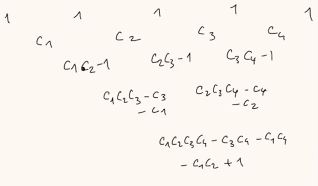
\includegraphics{./figures/L2.4}
  \end{figure}
  \item Item 4,
  \begin{ndefi}[Laurent Polynomial]
    $\frac{P(x_1, x_2, x_3, \dots x_w)}{x_1^{k_1}x_2^{k_2}\dots x_w^{k_w}}$
  \end{ndefi}
  and if consider a zig zag, all we are going os just saying we are considering things to the left or right and below your current position.
\end{itemize}

\begin{proof}[Proof of Thm 1]
  Start with a Conway-Coxeter frieze and call the values of the first row $\dots, c_0, c_1, \dots, (c_i)_{i\in\Z}$. We fix three consecutive diagonals.
  \begin{figure}[!ht]
    \centering
    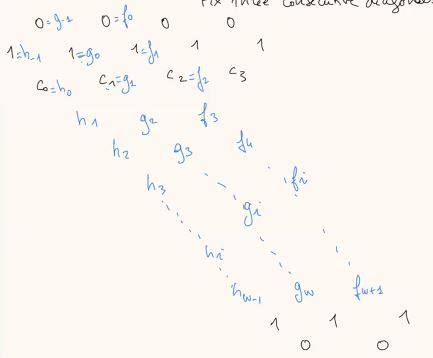
\includegraphics{./figures/L2.5}
  \end{figure}
  \newpage
  \begin{lemma}
    $\frac{f_i + h_i}{g_i} = K$
  \end{lemma}
  \begin{proof}
    Apply the frieze rule round these values and get,
    \begin{align*}
      1 &= g_i f_{i+1} - f_ig_{i+1}\\
      1  &= h_ig_{i+1} - g_ih_{i+1}\\
        g_if_{i+1} + g_ih_{i+1} &= h_ig_{i+1} + f_{i}g_{i+1}\\
        \frac{f_{i+1}h_{i+1}}{g_{i+1}} &= \frac{f_{i}h_{i}}{g_{i}}
    \end{align*}
    and so we can see,
    \begin{align*}
      \frac{f_0+h_0}{g_0} &= \frac{f_{w+1} + h_{w+1}}{g_{w+1}}\\
      c_0 &= f_{w+1}
    \end{align*}
    and so we have that we have a type of glide symmetry.
  \end{proof}
  Now using identical argument, we can start to determine more of the frieze. Hence, we have proved the glide symmetry. Now, we have also proved (1), which is implied by (2).\\

  We are going to take diagonals in the other direction and use similar arguments, we will find that,
  $$ \frac{h_0+h_2}{h_1} = \frac{g_0 + g_2}{g_1} = \frac{f_0 + f_2}{f_1} = c_2 $$
  and hence, we obtain the recurrance relation of,
  $$ g_i = c_ig_{i-1} - g_{i-2} $$
  This is the key lemma for the big proof. If $g_{i-1}$ and $g_{i-2}$ are polynomials in $c$, then so is $g_i$. Now, we have proved (3). \\

  Finally, for (4), exercise 4 gives a proof and an explicit formula in the particular case of a diagonal. In the case of an arbitrary zig-zag, we don't know any elementary proof, the one I know is based on Cluster Algebra and Cluster Algebra. You can focus on elements of the frieze as cluster elements.
\end{proof}

\section{Proof of the Bijection Theorem}
We are going to prove the Bijection Theorem by induction,\\

\begin{nthm}[Conway-Coxeter]
  There is a bijection,
  $$ \{\text{freizes of $\Z_{>0}$}\} \longleftrightarrow \{\text{Triangulations of polygons with $w + 3$ polygons} \} $$
\end{nthm}

To go from an triangulated $n$ to a $n+1$-gon, just add a triangle. Our quiddity sequence goes,
$$ (c_1, c_2, c_3, \dots, c_{n-1}, c_n) \to (c_1, c_2, c_3, \dots, c_{n-1}+1, 1, c_n+1) $$
We will call this augmentation. In a quiddity sequence, there will always be a one. So, if we have an augmentation, we can remove a triangle and go the other way, this is called reduction.\\

We want to show that these two operations are well defined on the set of frieze.

\begin{nlemma}[]
  The first row of a frieze always contains a one.
\end{nlemma}

We need something to allow us to work out if a sequence works for a frieze, this is given by an equation,
\begin{equation}
  N(c_1, c_2, \dots, c_n) = \begin{pmatrix}
    0 & -1 \\ 1 & c_1
\end{pmatrix}\begin{pmatrix}
  0 & -1 \\ 1 & c_2
\end{pmatrix} \dots \begin{pmatrix}
  0 & -1 \\ 1 & c_n
\end{pmatrix}
\end{equation}

\begin{prop}
  $N(c_1, c_2, \dots, c_n) = N(c_1, c_2, \dots, c_{n-1} +1, 1, c_n + 1 ) $
\end{prop}

\begin{proof}
  Just need to check $N(c, d) = N(c+1, 1, d+1)$
\end{proof}

\begin{prop}
  $(c_1, c_2, \dots, c_n)$ defines the first row of a frieze if and only if, $N(c_1, c_2, \dots, c_n) = -\id$ and $N(c_1, c_2, \dots, c_i)$ has positive entries in the second row for all $i = 1, \dots, n-3$..
\end{prop}

\begin{remark}
  In Exercise 5, we use $M(c_1, \dots, c_n)$,
  $$ M(c_1, c_2, \dots, c_n) = \begin{pmatrix}
    c_1 & -1 \\ 1 & 0
\end{pmatrix}\begin{pmatrix}
  c_2 & -1 \\ 1 & 0
\end{pmatrix} \dots \begin{pmatrix}
  c_n & -1 \\ 1 & 0
\end{pmatrix} = ^TN(c_1, \dots, c_n)^{-1}$$
Lemma is Ex5.3 and Prop 2.
\end{remark}

So, where does the first part of Prop 2 come from? If we use the recurrence relation we derived last lecture,
\begin{recall}
  Recurrence Relations,
  $$ g_i = c_ig_{i-1}-g_{i-2} \qquad  g_{-1} = 0 \quad g_0 = 1$$
  $$ f_i = c_i f_{i-1} - f_{i-1} \qquad f_{-1} = -1 \quad f_0 = 0 $$
\end{recall}

Now write them as a matrix,
$$ \begin{pmatrix}
  f_{i-2} & f_{i-1} \\ g_{i-2} & g_{i-1}
\end{pmatrix}\begin{pmatrix}
  0 & -1 \\ 1 & c_i
\end{pmatrix} = \begin{pmatrix}
  f_{i-1} & f_{i} \\ g_{i-1} & g_{i}
\end{pmatrix} $$

which then gives us,
$$ \begin{pmatrix}
  0 & -1 \\ 1 & c_1
\end{pmatrix}\begin{pmatrix}
0 & -1 \\ 1 & c_2
\end{pmatrix} \dots \begin{pmatrix}
0 & -1 \\ 1 & c_i
\end{pmatrix} $$
and when $i = n (= w+ 3)$, we obtain,
$$ \begin{pmatrix}
  -1 & 0 \\ 0 & 1
\end{pmatrix} N(c_1, \dots, c_n) = \begin{pmatrix}
  1 & 0 \\ 0 & -1
\end{pmatrix}$$
and so,
$$ N(c_1, \dots, c_n) = -\id $$

You can prove the frieze rule and induction to prove that if one line of the frieze is positive, all of it is positive. This gives us positivity up to $n-2$. Now if we augment our sequence, then the augmented sequence shall also follow the lemma. It's completely equivalent.\\

\subsection{Triangulations and friezes}
We can say more about friezes and triangulations. take this frieze,
\begin{figure}[!ht]
\centering
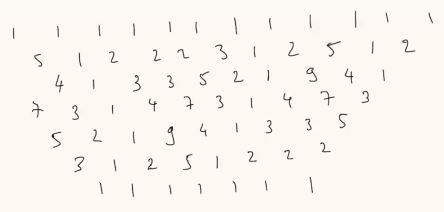
\includegraphics{./figures/L3.1}
\end{figure}

We can look at octogon, or we could extract a fundemental domain. We have a glide symmetry, so focus on a singular segment and focus on the ones.\\

Call the entries of the frieze,
\begin{figure}[!ht]
\centering
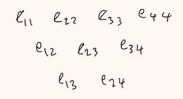
\includegraphics{./figures/L3.2}
\caption{}
\end{figure}

If $e_{ij} = 1$ then $i-1$ is connected to $j+1$.

and now consider continued fractions, if we take the triangulation from before, we can form a diagonal,
\begin{figure}[!ht]
\centering
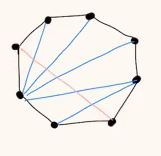
\includegraphics{./figures/L3.3}
\end{figure}

Now this associated with a rational number, which one? If we look at the triangles above and below the line.
$$ [1, 3, 1,1] = [1, 3, 2] = \lb 2, 2, 2, 3\rb $$

Then we can do the `Farey Sum', the sum

\begin{figure}[!ht]
\centering
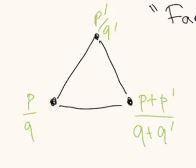
\includegraphics{./figures/L3.4}
\end{figure}

and do this over the on the polygon,

\begin{figure}[!ht]
\centering
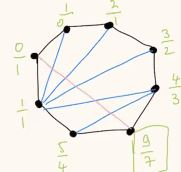
\includegraphics{./figures/L3.5}
\end{figure}

We can look at Farey Graphs,
% insert image
We can have all the rationals and we draw fractions on the edges, exactly when $pq' - p'q =\pm1$ for two rationals, $\frac{p}{q}$ and $\frac{p'}{q'}$. You can always carry on closer. It's a tesselation on the half plane with weird semi-circle tiles. To find the continued fraction, draw a vertical line and see what you cross, then take that finite picture. Play the game again, going from top down, then colour them from left and right. \\


\begin{figure}[!ht]
\centering
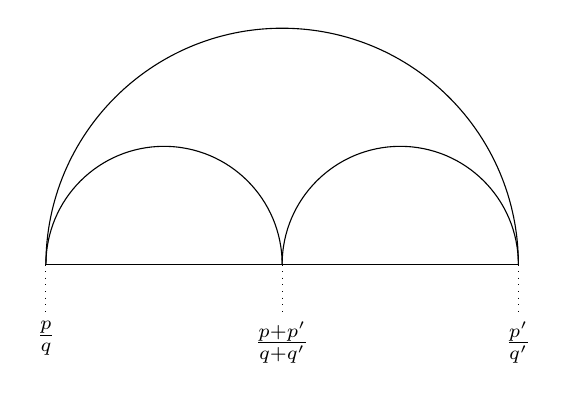
\begin{tikzpicture}[scale=6]
\draw (0,0) -- (1,0);
\draw (1,0) arc (0:180:.5);

\draw [dotted] (0,0) -- (0,-.1) node[below]{$\frac{p}{q}$};
\draw [dotted] (1,0) -- (1,-.1) node[below]{$\frac{p'}{q'}$};

\draw (1,0) arc (0:180:.25);
\draw [dotted] (.5,0) -- (.5,-.1) node[below]{$\frac{p+p'}{q+q'}$};
\draw (.5,0) arc (0:180:.25);

\end{tikzpicture}
\caption{Farey Sum Rule}
\end{figure}

Then if we take $\frac{7}{5}$, we can get $[1, 2, 1, 1]$ and then we can go from right to left and map that to a top bottom frieze.

\section{Tying up all the knots}
In this lecture Hirzebruch Formula, then Geometry of Friezes and New Developments and variants of friezes. We are going to go back and revisit things.\\

\subsection{Hirzebruch Formula}

\begin{nthm}[Hirzebruch Formula]
  $$ [a_1, a_2, a_3, \dots, a_n] = a_1 + \frac{1}{a_2 + \frac{1}{\ddots}} = c_1 - \frac{1}{c_2 - \frac{1}{c_3 - \frac{1}{\ddots}}}$$
\end{nthm}

\begin{claim}
  $$ [a_1, \dots, a_{2m}] = \llbracket a_1 + 1, 2,2, \dots, 2, a_3 + 2, \dots, 2, \dots, a_{2n-1} + 2, 2, \dots, 2\rrbracket $$
\end{claim}

This formula may be understood as a change of generators in the group $SL_2(2, \Z)$.

$$ T = \begin{matrix}
  1 & 1 \\ 0 & 1
\end{matrix} \qquad S = \begin{matrix}
  0 & -1 \\ 1 & 0
\end{matrix} \qquad L = \begin{matrix}
  1 & 0 \\ 1 & 1
\end{matrix}$$

\begin{fact}
  $$ SL(2, \Z) = \langle T, S \rangle  = \langle L, T \rangle $$
\end{fact}

If we consider $T^{c_1}ST^{c_2}S\dots T^{c_k}S = \begin{pmatrix}
  p & r \\ q & s
\end{pmatrix}$

\begin{fact}
  $$ \frac{p}{q} = \lb c_1, c_2, \dots, c_k \rb $$
\end{fact}
and so,
$$ T^{c_1}ST^{c_2}S\dots T^{c_k}S = T^{a_1}L^{a_2}T^{a_3}L^{a_4}\dots T^{a_{2n-1}}L^{a_{2m}} T^* $$
This can then be seen as our $N$ from the last lecture when we multiply by pairs. We can adjust the $*$ to make sure that the first $TS$ product makes the same as $TL$.

Now we make a matrix computation,
\begin{nlemma}[]
  $$ T^a = -M(a+1,1,1) $$
  $$ L^a = M(1, 2, 2, \dots, 1, 1) $$
  with $a$ 2's.\\
  $$ M(1, 1, 1) = -\id $$
  $$ M(2, 1,1, a+1) = M(a+2) $$
\end{nlemma}
\begin{proof}
  Trivial
\end{proof}

To get Hirzebruch Formula, just use the previous lemma and make a substitution,
$$ T^{a_1}L^{a_2} \dots = M(a+1, 1, 1) M(1, 2, 2, \dots, 2, 1, 1)\dots = M(a+1, 2, 2, \dots, 2, 1, 1)\dots $$

adding another,
$$ T^{a_1}L^{a_2}T^{a_3} \dots = M(a+1, 2, 2, \dots, 2, 1, 1)M(a_3 + 1, 1, 1)\dots = M(a+1, 2, 2, \dots, 2 a_3 +2, 2, 2, 2, \dots) $$

\newpage
\subsection{Geometry of friezes}
Friezes were ways to represent relationships between numbers in Geometric pictures.

\begin{figure}[!ht]
\centering
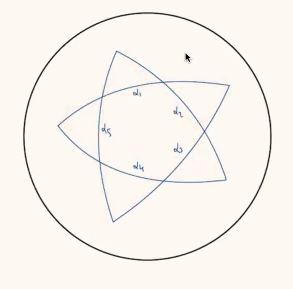
\includegraphics{./figures/L4.1}
\caption{Pentagram on a Sphere}
\end{figure}

Every line is on a great circle of the sphere and on the extremities we have right angles. In the 16$^{th}$, there was a question to find the analogous of pythagoras in spherical Geometry. \\

If we let $c_i = (\tan \a_i)^2$, then we get a frieze,
\begin{figure}[!ht]
\centering
\begin{tabular}{cccccccccc}
 1&&1&&1&&1&&1& \\
 &$c_1$&&$c_2$&&$c_3$&&$c_4$&&\\
 &&$c_4$&&$c_5$&&$c_1$&&$c_2$\\
 &1&&1&&1&&1&& \\
\end{tabular}
\end{figure}

$$ c_i c_{i+1} = 1 + c_{i+3} $$
describes this frieze. There is a cyclic symmetry and the above e1uation is true up to modulo 5.Hence the frieze is $5$ periodic.


\begin{nthm}[]
  If $(c_i)_{i \in \Z}$ such that $c_i \ne 0$ and
  $$ c_i c_{i+1} = 1 + c_{i+3} $$
  then $(c_i)$ is five periodic.
\end{nthm}

\begin{figure}[!ht]
\centering
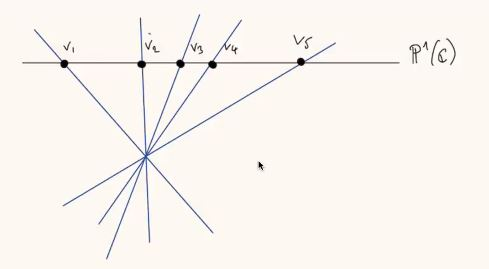
\includegraphics[width=0.4\textwidth]{./figures/L4.2}
\end{figure}

\newpage
We now want configurations of points modulo $PSL(2, \C)$, we can send three metric lines to any other three metric lines. For four lines, it's not always possible, we have to see if they are the same cross ratio.

Let,
$$ c_1 = (v_2, v_3, v_4, v_5) $$
$$ c_2 = (v_3, v_4, v_5, v_1) $$
$$ \vdots $$
$$ c_5 = (v_1, v_2, v_3, v_4) $$

and again, we get a frieze,
\begin{figure}[!ht]
\centering
\begin{tabular}{cccccccccc}
 1&&1&&1&&1&&1& \\
 &$c_1$&&$c_2$&&$c_3$&&$c_4$&&\\
 &&$c_4$&&$c_5$&&$c_1$&&\\
 &1&&1&&1&&1&& \\
\end{tabular}
\end{figure}

is a frieze.

$$  $$

This is then equivalent to the set of friezes over $\C \setminus \{0\}$ of width $n-3$.

\subsection{New Developments and Variants}
In 2005, there was revival of friezes due to their connection with Cluster Algebra. We can change the rule, why shouldn't we use other operations? We don't even need to use subtraction, so we can use tropical semifields,
$$ a \otimes d = b \otimes d \oplus 1 $$
and so we have a tropical frieze. We could just have addition,
$$ a + d = b + c $$
or nim addition,
$$ a \boxplus d = b \boxplus c +1 $$
We can work over $\F_q$, count how many friezes. We can change the configuration again with a middle value called a 2-frieze,
%    b
%  a e d
%    c
We can get rid of the bottom row and get infinite friezes or look at $SL(2, \Z)$ tilings. We can take bigger squares and look at $SL(k, \Z) / SL(k, \C)$.\\

We can link friezes to Cluster Algebra because of notation and Quivers.

\section{Misc}

\subsection{Quiver}
A quiver is an oriented graph, a collection of arrow. There aren't any loops. Arrows also only can go in one direction.

\[\begin{tikzcd}
	{x_1\\ \bullet} & {x_2\\ \bullet}
	\arrow[shift right=3, from=1-1, to=1-2]
\end{tikzcd}\]

We can consider a quiver mutation, you can change the graph locally.
\begin{itemize}
  \item You find a point.
  \item Add an arrow from i to j
  \item Reverse the arrows touching $k$
  \item Cancel the two loops, if any.
\end{itemize}

Quiver verticies can have a vertex attached to them and we can also mutate these variables.
$$ (x_1, x_2, \dots, x_n) $$
So we change $x_k$ to $x_k' = \frac{1}{x_k} \prod_{i \to k}x_i + \prod_{k \to j} x_j$\\

If we play this game with,

Then we can get a frieze out of this. they are exactly made out of the rule of mutations from the quiver,

\[\begin{tikzcd}
	{x_1\\\bullet} & {x_2\\\bullet} & \dots & {x_w\\\bullet}
	\arrow[shift left=3, from=1-4, to=1-3]
	\arrow[shift right=3, from=1-2, to=1-3]
	\arrow[shift right=3, from=1-1, to=1-2]
\end{tikzcd}\]

\subsection{Areas of research}
Friezes are a subset of Cluster Algebra, and they are used in combinatorics for triangle disections.

\end{document}
